\documentclass[preview]{standalone}
\usepackage{tikz,fullpage,tikz-network,verbatim}
\usetikzlibrary{arrows, petri, topaths, calc, angles, quotes}
\begin{document}
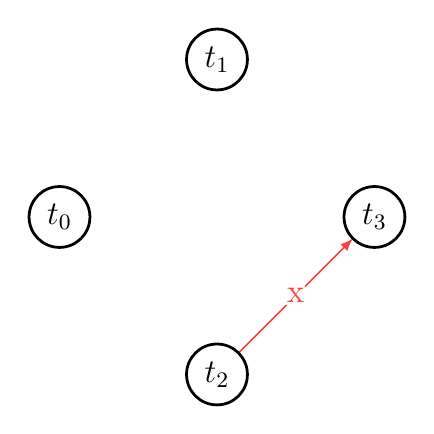
\begin{tikzpicture}[scale=1,transform shape]
  % \draw (0, 0) grid (6, 6);

  \SetVertexStyle[FillColor=white,TextFont=\large,MinSize=22]
  \Vertex[x=1,y=3,label=$t_0$]{t0}
  \Vertex[x=3,y=5,label=$t_1$]{t1}
  \Vertex[x=3,y=1,label=$t_2$]{t2}
  \Vertex[x=5,y=3,label=$t_3$]{t3}

  \SetEdgeStyle[TextFont=\large,LineWidth=0.6pt,InnerSep=0.5pt,Color=red!75]
  \Edge[label=x,Direct](t2)(t3)
\end{tikzpicture}
\end{document}
